% Provenance (never printed): cycle 4 SVT, "La planete Terre, l'environnement
% et l'action humaine": climate, its past variations and the present change,
% read from data; see sources/book1/PROVENANCE.md. Book 1, grade 9, chapter 1.
% Vocabulary guard: owns climate change (first look; Book 2 g12 re-uses it),
% global warming, temperature anomaly. The greenhouse effect and greenhouse
% gases belong to the chemistry series (grade 8): recalled in prose, never
% defined. Infrared is physics (g10): named in prose only. "Glacial period"
% and "interglacial" belong to Book 2 g12: here "the ice ages and the warmer
% times between them". Physical science only, in the IPCC's calibrated words;
% no policy.
\chapter{Iklim Bumi, Dahulu dan Sekarang}\label{ch:g9:climate-past-and-present}

Seandainya Bumi tidak dikelilingi udara, tetapi memantulkan bagian sinar
matahari yang sama seperti sekarang, permukaannya akan mencapai suhu
rata-rata sekitar \qty{-19}{\degreeCelsius}: \omterm{def:g2:water-on-earth:ocean}{laut} membeku, daratan
membeku, di mana-mana. Suhu rata-ratanya yang sebenarnya sekitar
\qty{15}{\degreeCelsius}. Selisihnya, sekitar \qty{34}{\degreeCelsius},
berasal dari beberapa gas di udara, yang jumlahnya sangat sedikit, yang
menahan sebagian panas Bumi agar tidak lepas ke antariksa. Bab ini
membahas gas-gas tersebut, \omterm{def:g5:weather-and-climate:climate}{iklim} Bumi pada masa lalu, serta bagaimana dan
mengapa \omterm{def:g5:weather-and-climate:climate}{iklim} itu berubah sekarang.
% ledger: earth:Tbb, earth:Tsurf (figdata/grade-9/climate_records.py: -19.1 and 14.9 degC, gap 34)

\begin{recall}
\omterm{def:g5:weather-and-climate:climate}{Iklim} suatu tempat adalah \omterm{def:g1:watching-the-weather:weather}{cuaca} yang biasa dialaminya, dirata-ratakan
selama 30 tahun (\cref{ch:g5:weather-and-climate}). Lapisan terbawah
atmosfer, tempat \omterm{def:g1:watching-the-weather:weather}{cuaca} terjadi, adalah \omterm{def:g8:the-atmosphere:layers}{troposfer}
(\cref{ch:g8:the-atmosphere}). \omterm{def:g8:ice-on-earth:ice-age}{Zaman es}, dengan \omterm{def:g8:ice-on-earth:ice-sheet}{lapisan es} yang meluas
jauh melampaui \omterm{def:g3:continents-and-oceans:poles}{kutub}, telah datang dan pergi; \omterm{def:g8:ice-on-earth:sea-ice}{es laut} Arktik telah
menyusut sejak tahun 1979 (\cref{ch:g8:ice-on-earth}). Dalam kimia, kamu
belajar bahwa karbon dioksida, metana, dan uap air adalah \emph{gas rumah
kaca}: gas-gas itu meneruskan sinar matahari, tetapi menyerap cahaya
inframerah yang tidak kasatmata yang dipancarkan oleh tanah yang hangat,
dan itulah \emph{efek rumah kaca}; pembakaran batu bara, minyak bumi, dan
gas alam melepaskan karbon dioksida.
\end{recall}

\section{Efek rumah kaca dan suhu Bumi}

Sinar matahari menembus atmosfer dan memanaskan tanah dan \omterm{def:g2:water-on-earth:ocean}{samudra}. Seperti
setiap benda yang hangat, permukaan yang hangat itu pada gilirannya
memancarkan energi, berupa cahaya inframerah yang tidak dapat dilihat
mata. Seandainya semuanya lepas ke antariksa, Bumi akan menjadi dunia
beku seperti dalam paragraf pertama. Namun, gas-gas rumah kaca di udara
menyerap sebagian besar cahaya inframerah ini dan mengirimkan sebagiannya
kembali ke bawah: permukaan menerima energi dari Matahari sekaligus dari
udara di atasnya, sehingga mencapai suhu yang lebih tinggi.

\begin{omfigure}
\begin{tikzpicture}[font=\footnotesize, >={Stealth[length=2.4mm]}]
  % ground and atmosphere
  \fill[omLithAlluv] (0,0) rectangle (12,0.5);
  \fill[omSea!45] (0,0.5) rectangle (12,3.4);
  \node[anchor=north east, align=right] at (11.85,3.35) {atmosfer dengan\\ gas rumah kaca};
  \node[anchor=south east] at (11.9,0.05) {tanah dan samudra};
  \node[anchor=south west] at (0.15,3.5) {antariksa};
  % Sun
  \fill[omWxSun] (1.3,5.0) circle (0.45);
  \node[anchor=east] at (0.8,5.0) {Matahari};
  % sunlight in
  \draw[->, omWxSun!80!black, line width=2.2pt] (1.7,4.6) -- (2.7,0.55)
    node[pos=0.25, right=2pt, align=left, black] {sinar matahari masuk\\ dan memanaskan permukaan};
  % infrared out and back
  \draw[->, omWarm, line width=1.6pt, decorate, decoration={snake, amplitude=1mm, segment length=4mm, post length=3mm}]
    (6.0,0.55) -- (6.6,2.6);
  \draw[->, omWarm, line width=1.6pt, decorate, decoration={snake, amplitude=1mm, segment length=4mm, post length=3mm}]
    (6.6,2.7) -- (7.4,5.0) node[right, align=left, black] {sebagian lepas\\ ke antariksa};
  \draw[->, omWarm, line width=1.6pt, decorate, decoration={snake, amplitude=1mm, segment length=4mm, post length=3mm}]
    (6.8,2.75) -- (8.6,0.55);
  \node[align=left, anchor=west] at (8.8,1.9) {sebagian diserap\\ oleh gas-gas itu dan\\ dikirim kembali ke bawah};
  \node[align=right, anchor=east] at (5.9,1.3) {permukaan yang\\ hangat memancarkan\\ inframerah};
\end{tikzpicture}

{\small Efek rumah kaca, secara sederhana (sketsa). Tanpa efek ini, suhu
rata-rata permukaan Bumi sekitar \qty{-19}{\degreeCelsius}; dengan efek
ini, sekitar \qty{15}{\degreeCelsius}.}
% ledger: earth:Tbb, earth:Tsurf
\label{fig:g9:climate-past-and-present:greenhouse}
\end{omfigure}

Efek rumah kaca bersifat alami dan diperlukan: tanpanya tidak akan ada air
cair di permukaan. Pertanyaan bab ini lain lagi: apa yang terjadi pada
suhu Bumi ketika jumlah gas rumah kaca di udara berubah?

\section{Iklim masa lalu}

Untuk membaca \omterm{def:g5:weather-and-climate:climate}{iklim} masa lalu yang jauh, para ilmuwan mengebor \omterm{def:g8:ice-on-earth:ice-sheet}{lapisan es}.
Setiap tahun, \omterm{def:g4:clouds-rain-snow:precipitation}{salju} turun di Antarktika dan Greenland, dan \omterm{def:g4:clouds-rain-snow:precipitation}{salju} musim
panas sedikit berbeda dari \omterm{def:g4:clouds-rain-snow:precipitation}{salju} musim dingin. Setelah terkubur dan
tertekan menjadi es, lapisan-lapisan tahunan itu tetap ada, yang satu di
atas yang lain, seperti halaman-halaman sebuah buku. Makin dalam esnya,
makin tua umurnya.
% ledger: eo:ice-core

\begin{omfigure}
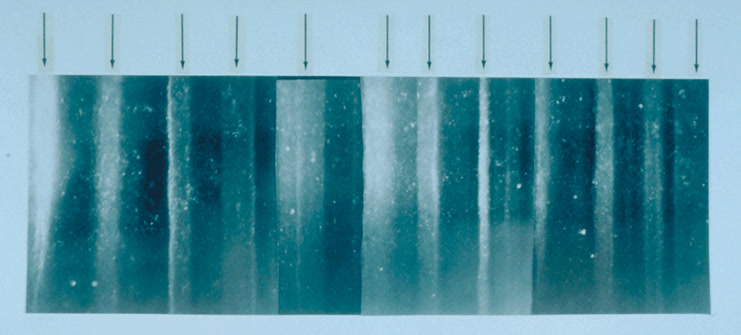
\includegraphics[width=0.78\linewidth]{images/book1/g9-gisp2-layers.jpg}

{\small Sepotong inti es sepanjang \qty{19}{cm}, yang dibor pada kedalaman
\qty{1855}{m} di \omterm{def:g8:ice-on-earth:ice-sheet}{lapisan es} Greenland dan disinari dari bawah. Panah-panah
menunjuk lapisan musim panas yang lebih terang, di antara lapisan musim
dingin yang lebih gelap: \omterm{def:g4:clouds-rain-snow:precipitation}{salju} selama sebelas tahun. NOAA Paleoclimatology
(domain publik, melalui Wikimedia Commons).}
% ledger: commons:gisp2-layers
\label{fig:g9:climate-past-and-present:ice-core}
\end{omfigure}

Inti es menyimpan dua catatan masa lalu. \omterm{def:g4:clouds-rain-snow:precipitation}{Salju} itu sendiri menunjukkan
seberapa dingin udara ketika \omterm{def:g4:clouds-rain-snow:precipitation}{salju} itu turun: makin dingin udaranya, makin
kecil bagian bentuk hidrogen dan oksigen yang lebih berat di dalam \omterm{def:g4:clouds-rain-snow:precipitation}{salju}.
Selain itu, selagi \omterm{def:g4:clouds-rain-snow:precipitation}{salju} tertekan menjadi es, ruang di antara
butir-butirnya menutup dan memerangkap gelembung-gelembung kecil udara
pada masa itu. Para ilmuwan melepaskan udara purba ini di laboratorium dan
mengukur karbon dioksidanya.
% ledger: eo:ice-core

\begin{omfigure}
\begin{tikzpicture}
\begin{axis}[name=temp, omrecord, omage, width=13cm, height=3.9cm, xmin=0, xmax=800,
  xtick={0,100,...,800}, xticklabels={}, ylabel={perubahan\\ suhu ($^\circ$C)},
  ylabel style={align=center}, ymin=-11, ymax=5, ytick={-10,-5,0,5}]
  \addplot[omWarm, line width=0.7pt] table[x=age_kyr, y=temp_C] {figdata/out/grade-9-climate_records-edc.dat};
\end{axis}
\begin{axis}[at={(temp.south west)}, anchor=north west, yshift=-0.3cm, omrecord, omage,
  width=13cm, height=3.9cm, xmin=0, xmax=800, xtick={0,100,...,800},
  xlabel={ribuan tahun sebelum sekarang}, ylabel={karbon dioksida\\ (ppm)},
  ylabel style={align=center}, ymin=160, ymax=320, ytick={180,220,260,300}]
  \addplot[black, line width=0.7pt] table[x=age_kyr, y=co2_ppm] {figdata/out/grade-9-climate_records-icecore.dat};
\end{axis}
\end{tikzpicture}

{\small Delapan ratus ribu tahun yang dibaca di dalam es Antarktika. Atas:
perubahan suhu udara di Dome~C, dibandingkan dengan rata-rata seribu tahun
terakhir (inti es EPICA Dome~C, J.~Jouzel dan kawan-kawan, 2007). Bawah:
karbon dioksida di udara yang terperangkap di dalam es, dalam bagian per
sejuta (B.~Bereiter dan kawan-kawan, 2015). Keduanya dirata-ratakan per
langkah \num{2000} tahun; waktu berjalan dari kiri (paling tua) ke kanan
(sekarang).}
% ledger: data:edc-jouzel, data:co2-bereiter (figdata/grade-9/climate_records.py)
\label{fig:g9:climate-past-and-present:icecore}
\end{omfigure}

Kedua kurva itu menceritakan kisah yang sama. Berulang kali, masa dingin
yang panjang, yaitu \omterm{def:g8:ice-on-earth:ice-age}{zaman es}, berganti dengan masa hangat yang lebih
pendek, lalu dingin datang kembali. Pada saat terdingin, udara di atas
Antarktika sekitar \qty{9}{\degreeCelsius} lebih dingin daripada pada
seribu tahun terakhir; pada masa terhangat, udaranya beberapa derajat
lebih hangat. Karbon dioksida pun naik turun bersama suhu, antara sekitar
\qty{175}{ppm} pada masa dingin dan sekitar \qty{300}{ppm} pada masa
hangat. Kita hidup di salah satu masa hangat, yang dimulai ketika \omterm{def:g8:ice-on-earth:ice-age}{zaman es}
terakhir berakhir.
% ledger: data:edc-jouzel, data:co2-bereiter (figdata/grade-9/climate_records.py: edc min -9.7, max +3.6; CO2 174 to 299 ppm)

\begin{method}[Membaca dua catatan berdampingan]
\begin{enumerate}
  \item Periksalah apakah kedua catatan memakai sumbu waktu yang sama, dan
        ke arah mana waktu berjalan.
  \item Pilihlah satu tanggal pada sumbu waktu dan bacalah setiap catatan
        pada tanggal itu.
  \item Carilah puncak dan \omterm{def:g1:landscapes-around-us:landform}{lembahnya}: apakah keduanya muncul pada waktu
        yang sama di kedua catatan?
  \item Katakan apa yang bergerak bersama-sama, tanpa memutuskan dulu
        perubahan mana yang menyebabkan perubahan yang lain.
\end{enumerate}
\end{method}

\begin{example}[Zaman es terakhir di dalam inti es]
Pada \num{20000} tahun sebelum sekarang (angka 20 pada sumbu waktu),
kurva suhu berada di sekitar \qty{-9}{\degreeCelsius} dan karbon dioksida
di sekitar \qty{190}{ppm}. Pada seribu tahun terakhir, kurva suhu dekat
dengan 0 dan karbon dioksida dekat dengan \qty{280}{ppm}. Jadi, pada saat
terdingin \omterm{def:g8:ice-on-earth:ice-age}{zaman es} terakhir, udara di atas Antarktika sekitar
\qty{9}{\degreeCelsius} lebih dingin, dan mengandung
$280 - 190 = \qty{90}{ppm}$ karbon dioksida lebih sedikit, sepertiga
lebih sedikit.
\end{example}
% ledger: data:edc-jouzel, data:co2-bereiter (figdata/grade-9/climate_records.py: 19-21 kyr bins -9.4, 190 ppm; 1 kyr bin 278)

Lebih jauh lagi ke masa lalu, Bumi pernah mengalami \omterm{def:g5:weather-and-climate:climate}{iklim} yang jauh lebih
hangat daripada \omterm{def:g5:weather-and-climate:climate}{iklim} mana pun selama 800\,000 tahun terakhir. Kajian-kajian
ilmiah memperkirakan bahwa terakhir kali permukaan Bumi bertahan
\qty{2.5}{\degreeCelsius} atau lebih di atas tingkatnya pada akhir abad
ke-19 adalah lebih dari tiga juta tahun yang lalu.
% ledger: ipcc:3myr

\section{Catatan masa kini}

Sejak akhir abad ke-19, suhu diukur setiap hari di ribuan \omterm{def:g4:clouds-rain-snow:weather-station}{stasiun cuaca}
di darat dan di \omterm{def:g2:water-on-earth:ocean}{laut}, dengan termometer yang disimpan di tempat teduh.
Untuk mengikuti seluruh planet, para ilmuwan tidak merata-ratakan suhunya
sendiri, yang bergantung pada letak setiap stasiun, melainkan seberapa
jauh setiap suhu berbeda dari nilai biasanya sendiri.
% ledger: giss:method

\begin{definition}[Anomali suhu]\label{def:g9:climate-past-and-present:anomaly}
Yang disebut \emph{anomali suhu}\index{anomali suhu} adalah selisih
antara suatu suhu dan rata-ratanya selama suatu periode acuan yang
dipilih. Anomali itu positif jika suhunya lebih hangat daripada
rata-rata itu, negatif jika lebih dingin.
\end{definition}

\begin{omfigure}
\begin{minipage}[c]{0.44\linewidth}\centering
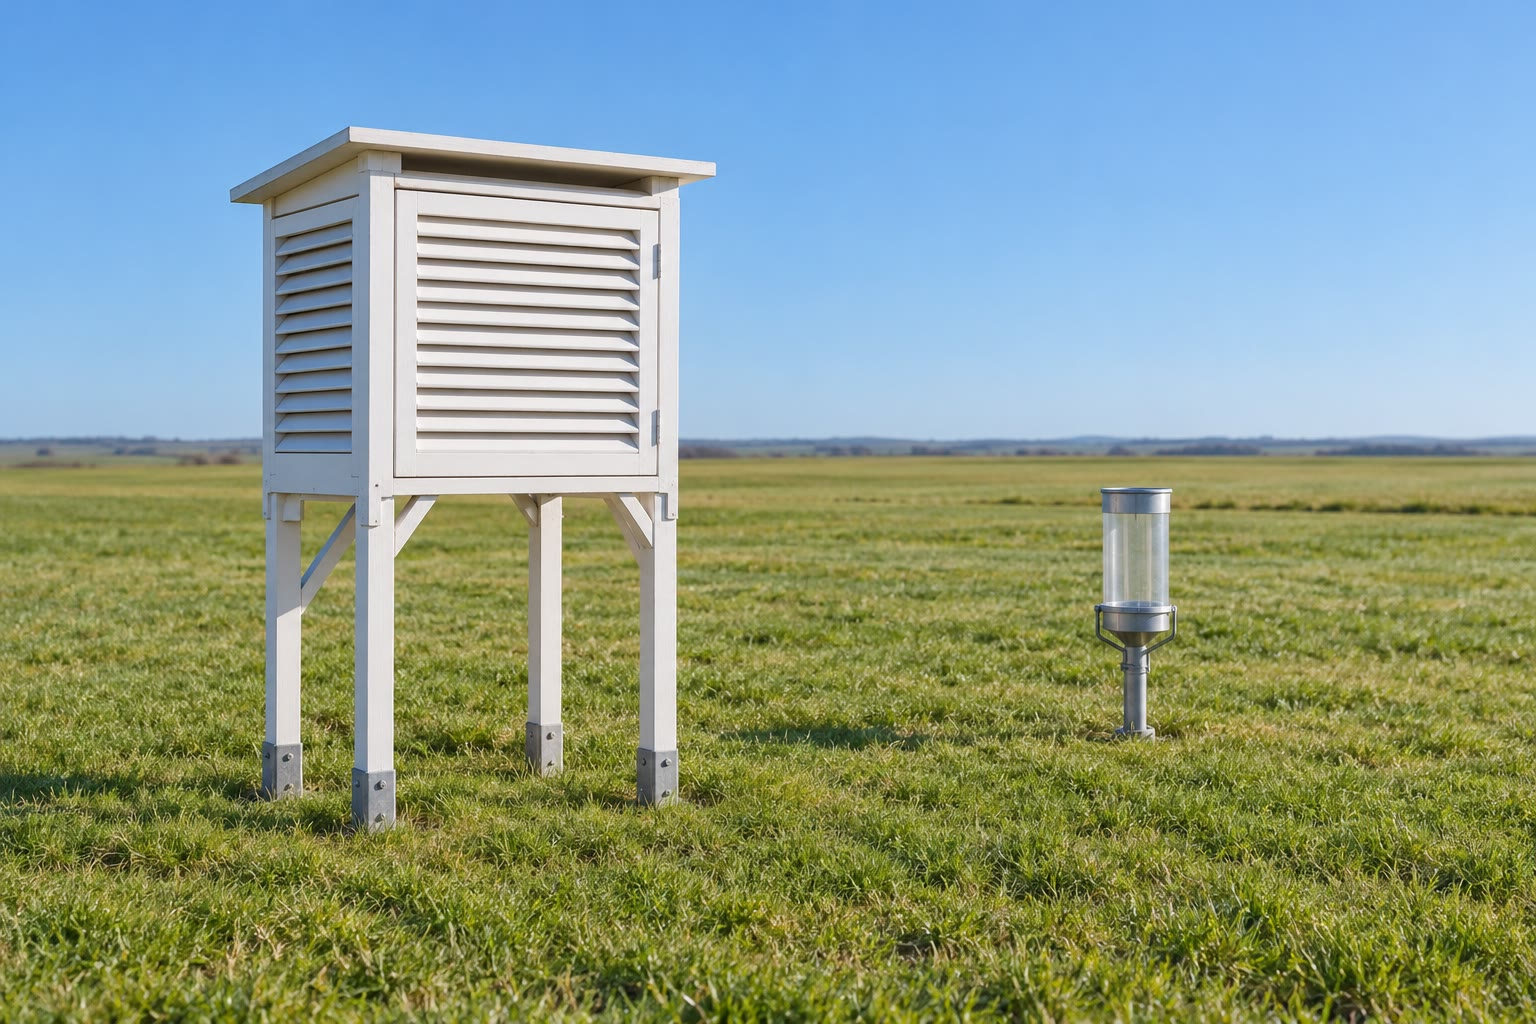
\includegraphics[width=\linewidth]{images/book1/ai/g9-weather-screen.jpg}
\end{minipage}\hfill
\begin{minipage}[c]{0.52\linewidth}\raggedright
{\small Sebuah \omterm{def:g4:clouds-rain-snow:weather-station}{stasiun cuaca}: kotak putih berkaki dengan dinding
berkisi-kisi, yaitu sangkar meteorologi, menjaga termometer tetap teduh
sementara udara mengalir melewatinya; di kanan, sebuah \omterm{def:g4:clouds-rain-snow:rain-gauge}{penakar hujan}
(ilustrasi AI dari suatu adegan umum).}
\end{minipage}
\label{fig:g9:climate-past-and-present:screen}
\end{omfigure}

Catatan suhu global NASA, misalnya, memberikan anomali setiap tahun
dibandingkan dengan rata-rata 1951--1980, dari stasiun-stasiun darat dan
dari pengukuran \omterm{def:g4:world-physical-map:altitude}{permukaan laut}. Jika dirata-ratakan per dasawarsa, catatan
itu menunjukkan kenaikan yang jelas.
% ledger: giss:method, data:gistemp

\begin{omfigure}
\begin{tikzpicture}
\begin{axis}[omrecord, ybar, width=13cm, height=5.6cm, bar width=9pt,
  ymin=-0.45, ymax=1.2, ytick={-0.4,0,0.4,0.8,1.2},
  xtick=data, xticklabels={1880-an, 1890-an, 1900-an, 1910-an, 1920-an, 1930-an, 1940-an, 1950-an, 1960-an, 1970-an, 1980-an, 1990-an, 2000-an, 2010-an, 2020--2025},
  x tick label style={rotate=60, anchor=east, font=\scriptsize},
  ylabel={anomali suhu ($^\circ$C)}, xmajorgrids=false]
  \addplot[fill=omWarm!70, draw=black!50] table[x expr=\coordindex, y=mean_C]
    {figdata/out/grade-9-climate_records-decades.dat};
\end{axis}
\end{tikzpicture}

{\small Suhu permukaan global, per dasawarsa sejak tahun 1880-an, sebagai
anomali dibandingkan dengan rata-rata 1951--1980; batang terakhir mencakup
enam tahun 2020--2025. Data: NASA GISTEMP versi~4.}
% ledger: data:gistemp (figdata/grade-9/climate_records.py)
\label{fig:g9:climate-past-and-present:decades}
\end{omfigure}

\begin{definition}[Pemanasan global]\label{def:g9:climate-past-and-present:global-warming}
Yang disebut \emph{pemanasan global}\index{pemanasan global} adalah
kenaikan suhu rata-rata permukaan Bumi, secara keseluruhan, sejak
paruh kedua abad ke-19.
\end{definition}

Dari tahun ke tahun, catatan itu naik turun: satu tahun bisa lebih sejuk
daripada tahun sebelumnya, karena \omterm{def:g1:watching-the-weather:weather}{cuaca} selama satu tahun penuh, di atas
\omterm{def:g2:water-on-earth:ocean}{samudra} dan \omterm{def:g3:continents-and-oceans:continent}{benua}, juga berubah-ubah. Karena itu, untuk mengukur
pemanasan, para ilmuwan membandingkan rata-rata selama banyak tahun,
tidak pernah dua tahun saja.

\begin{omfigure}
\begin{tikzpicture}
\begin{axis}[omrecord, width=13cm, height=5.4cm, xmin=1875, xmax=2030, ymin=-0.6, ymax=1.4,
  xtick={1880,1900,...,2020}, x tick label style={/pgf/number format/1000 sep={}},
  xlabel={tahun}, ylabel={anomali suhu ($^\circ$C)},
  legend style={at={(0.2,0.97)}, anchor=north west, draw=none, fill=white, font=\footnotesize}]
  \fill[omWarm!10] (axis cs:1880,-0.6) rectangle (axis cs:1899,1.4);
  \fill[omWarm!10] (axis cs:2015,-0.6) rectangle (axis cs:2024,1.4);
  \addplot[black!70, mark=*, mark size=0.9pt, line width=0.4pt]
    table[x=year, y=anomaly_C] {figdata/out/grade-9-climate_records-annual.dat};
  \addlegendentry{setiap tahun}
  \addplot[omWarm, line width=2pt] table[x=year, y=mean_C] {figdata/out/grade-9-climate_records-periods.dat};
  \addlegendentry{rata-rata suatu periode}
  \draw[dashed, black!50] (axis cs:1875,0) -- (axis cs:2030,0);
  \node[font=\scriptsize, fill=white, inner sep=1pt] at (axis cs:1889.5,0.45) {1880--1899};
  \node[font=\scriptsize, fill=white, inner sep=1pt] at (axis cs:2019.5,0.3) {2015--2024};
\end{axis}
\end{tikzpicture}

{\small \omterm{def:g9:climate-past-and-present:anomaly}{Anomali suhu} global setiap tahun dari 1880 sampai 2025
(dibandingkan dengan rata-rata 1951--1980, garis putus-putus), dengan
rata-rata dua periode dari soal bab ini: 1880--1899 dan 2015--2024. Data:
NASA GISTEMP versi~4.}
% ledger: data:gistemp (figdata/grade-9/climate_records.py)
\label{fig:g9:climate-past-and-present:annual}
\end{omfigure}

\begin{method}[Mengukur pemanasan di antara dua periode]
\begin{enumerate}
  \item Pilihlah dua periode yang masing-masing sekurang-kurangnya sepuluh
        tahun, satu di awal dan satu di akhir, agar naik turunnya
        tahun-tahun tunggal saling meniadakan.
  \item Rata-ratakan anomali tahunan setiap periode.
  \item Kurangkan rata-rata awal dari rata-rata akhir: hasilnya adalah
        pemanasan di antara kedua periode itu, dalam derajat.
  \item Sebutkan catatan dan periode mana yang kamu pakai: catatan lain,
        atau periode lain, memberikan angka yang sedikit berbeda.
\end{enumerate}
\end{method}

\begin{example}[Pemanasan sejak tahun 1970-an]
Dalam catatan NASA, anomali sepuluh tahun 1970--1979 rata-rata
\qty{0.03}{\degreeCelsius}, dan anomali 2010--2019 rata-rata
\qty{0.80}{\degreeCelsius}. Pemanasan di antara kedua dasawarsa itu adalah
$0.80 - 0.03 = \qty{0.77}{\degreeCelsius}$, dalam empat puluh tahun:
sekitar \qty{0.19}{\degreeCelsius} per dasawarsa. Tahun-tahun tunggal,
yang juga berselang empat puluh tahun, akan memberikan jawaban yang sangat
berbeda: 1976 ($-0.10$) dibandingkan dengan 2016 (1.01) memberikan
\qty{1.11}{\degreeCelsius}, tetapi 1979 (0.16) dibandingkan dengan 2011
(0.61) hanya memberikan \qty{0.45}{\degreeCelsius}.
\end{example}
% ledger: data:gistemp (figdata/grade-9/climate_records.py: decade_1970s 0.03, decade_2010s 0.80; annual 1976 -0.10, 2016 1.01, 1979 0.16, 2011 0.61)

Karbon dioksida di udara telah diukur secara langsung sejak bulan Maret
1958, di sebuah observatorium sekitar \qty{3400}{m} di lereng \omterm{def:g4:volcanoes-earthquakes-first-look:volcano}{gunung api}
Mauna Loa, di Hawaii. Pada tahun 1959, rata-rata tahunannya
\qty{316}{ppm}; pada tahun 2025, nilainya sudah mencapai \qty{427}{ppm},
jauh di atas \qty{300}{ppm} yang tidak pernah dilampauinya selama
800\,000 tahun yang tercatat dalam es. Kenaikannya makin lama makin cepat:
kurang dari \qty{1}{ppm} setahun pada tahun 1960-an, lebih dari
\qty{2.5}{ppm} setahun dalam sepuluh tahun terakhir.
% ledger: gml:keeling, data:co2-mlo, data:co2-bereiter (figdata/grade-9/climate_records.py: 315.98, 427.35, 0.86 and 2.63 ppm/yr; ice core max 298.6)

\begin{omfigure}
\begin{tikzpicture}
\begin{axis}[omrecord, width=12cm, height=5cm, xmin=1955, xmax=2030,
  ymin=290, ymax=440, ytick={300,350,400}, xtick={1960,1970,...,2020},
  x tick label style={/pgf/number format/1000 sep={}},
  xlabel={tahun}, ylabel={karbon dioksida (ppm)}]
  \addplot[black, line width=0.9pt, mark=*, mark size=0.8pt] table[x=year, y=co2_ppm] {figdata/out/grade-9-climate_records-co2.dat};
  \draw[dashed, omWarm] (axis cs:1955,300) -- (axis cs:2030,300);
\end{axis}
\end{tikzpicture}

{\small Karbon dioksida di udara di Mauna Loa, Hawaii, rata-rata tahunan
1959--2025 (NOAA Global Monitoring Laboratory dan Scripps Institution of
Oceanography). Garis putus-putus pada \qty{300}{ppm} kira-kira merupakan
tingkat tertinggi yang ditemukan dalam 800\,000 tahun es Antarktika.}
% ledger: data:co2-mlo, data:co2-bereiter (figdata/grade-9/climate_records.py)
\label{fig:g9:climate-past-and-present:co2}
\end{omfigure}

\begin{dated}{2025}
Rata-rata tahunan karbon dioksida di Mauna Loa adalah \qty{427.35}{ppm}
pada tahun 2025. Dalam catatan NASA, tahun terhangat sejak 1880 adalah
2024, dengan anomali \qty{1.28}{\degreeCelsius} dibandingkan dengan
1951--1980.
% ledger: data:co2-mlo, data:gistemp (figdata/grade-9/climate_records.py)
\end{dated}

\omterm{def:g4:world-physical-map:altitude}{Permukaan laut} juga naik. Sejak tahun 1993, satelit telah mengukur
\omterm{def:g4:world-physical-map:altitude}{ketinggian} \omterm{def:g4:world-physical-map:altitude}{permukaan laut} di seluruh dunia: garis tren catatannya naik
sekitar \qty{3.2}{mm} setahun, sekitar \qty{10}{cm} dalam tiga puluh
tahun. Ada dua hal yang menaikkan \omterm{def:g4:world-physical-map:altitude}{permukaan laut}: air yang menghangat
memuai, dan es daratan yang mencair menambahkan air ke \omterm{def:g2:water-on-earth:ocean}{samudra}. Dan es
memang menyusut: \omterm{def:g8:ice-on-earth:glacier}{gletser-gletser} \omterm{def:g1:landscapes-around-us:landform}{gunung} hampir di mana-mana sedang mundur,
dan \omterm{def:g8:ice-on-earth:sea-ice}{es laut} musim panas di Arktik telah kehilangan hampir separuh luas
sebarannya sejak tahun 1979 (\cref{ch:g8:ice-on-earth}).
% ledger: data:gmsl-lsa (figdata/grade-9/climate_records.py: 3.18 mm/yr; 101 mm 1993-2024), ipcc:b1-ice, nsidc:ice-shelves, data:b1-nsidc-sea-ice

\begin{omfigure}
\begin{tikzpicture}
\begin{axis}[omrecord, width=12cm, height=4.8cm, xmin=1992, xmax=2026,
  ymin=-30, ymax=100, xtick={1995,2000,...,2025},
  x tick label style={/pgf/number format/1000 sep={}},
  xlabel={tahun}, ylabel={permukaan laut (mm)},
  legend style={at={(0.02,0.97)}, anchor=north west, draw=none, fill=white, font=\footnotesize}]
  \addplot[omCold, mark=*, mark size=1.1pt, line width=0.6pt] table[x=year, y=gmsl_mm] {figdata/out/grade-9-climate_records-sea.dat};
  \addlegendentry{rata-rata tahunan}
  \addplot[omWarm, dashed, line width=0.9pt] table[x=year, y=gmsl_mm] {figdata/out/grade-9-climate_records-sea-trend.dat};
  \addlegendentry{garis tren}
\end{axis}
\end{tikzpicture}

{\small \omterm{def:g4:world-physical-map:altitude}{Permukaan laut} rata-rata global yang diukur oleh satelit, rata-rata
tahunan 1993--2024, dibandingkan dengan suatu tingkat acuan, beserta garis
trennya (NOAA Laboratory for Satellite Altimetry).}
% ledger: data:gmsl-lsa (figdata/grade-9/climate_records.py)
\label{fig:g9:climate-past-and-present:sea}
\end{omfigure}

\section{Perubahan iklim dan penyebabnya}

\begin{definition}[Perubahan iklim]\label{def:g9:climate-past-and-present:climate-change}
Yang disebut \emph{perubahan iklim}\index{perubahan iklim} adalah
perubahan \omterm{def:g5:weather-and-climate:climate}{iklim} Bumi, atau \omterm{def:g5:weather-and-climate:climate}{iklim} suatu wilayah, yang berlangsung selama
puluhan tahun atau lebih: perubahan suhu rata-ratanya, \omterm{def:g4:clouds-rain-snow:precipitation}{hujannya},
anginnya, atau esnya, bukan sekadar satu musim yang tidak biasa.
\end{definition}

\omterm{def:g5:weather-and-climate:climate}{Iklim} selalu berubah, seperti yang ditunjukkan inti es. Yang baru adalah
kecepatan perubahan masa kini, dan penyebabnya. Para ilmuwan dari seluruh
dunia secara berkala menilai apa yang telah diterbitkan tentang \omterm{def:g5:weather-and-climate:climate}{iklim},
dalam laporan-laporan Panel Antarpemerintah tentang Perubahan \omterm{def:g5:weather-and-climate:climate}{Iklim}
(IPCC). Laporan-laporan itu menimbang seberapa pasti setiap pernyataan,
dengan kata-kata yang dipilih secara cermat.

Dalam laporan-laporan ini, setiap kata di bawah mempunyai arti yang
tetap: peluang dari 100 bahwa pernyataan itu benar.

\begin{center}
{\small
\begin{tabular}{|l|c||l|c|}
\hline
\emph{hampir pasti} & 99 sampai 100 & \emph{mungkin} & 66 sampai 100 \\
\emph{amat sangat mungkin} & 95 sampai 100 & \emph{sama mungkinnya dengan tidak} & 33 sampai 66 \\
\emph{sangat mungkin} & 90 sampai 100 & \emph{kecil kemungkinannya} & 0 sampai 33 \\
\hline
\end{tabular}}
\end{center}
% ledger: ipcc:likelihood

\noindent Beberapa pernyataan tidak memakai satu pun kata ini: pernyataan
itu diberikan sebagai fakta, misalnya ``hal itu \emph{tidak
terbantahkan}''. Ketika kamu membaca berita tentang \omterm{def:g5:weather-and-climate:climate}{iklim}, carilah
kata-kata ini, dan perhatikan mana yang dipertahankan berita itu dan mana
yang dibuangnya.
% ledger: ipcc:unequivocal

Kajian yang diterbitkan pada tahun 2021 menyatakan hal-hal berikut.
\begin{itemize}
  \item \emph{Tidak terbantahkan} bahwa pengaruh manusia telah
        menghangatkan atmosfer, \omterm{def:g2:water-on-earth:ocean}{samudra}, dan daratan.
  \item Suhu permukaan global pada 2011--2020 sekitar
        \qty{1.1}{\degreeCelsius} lebih tinggi daripada pada 1850--1900,
        dan masing-masing dari empat dasawarsa terakhir lebih hangat
        daripada dasawarsa mana pun sebelumnya sejak 1850.
  \item Pemanasan akibat manusia dari 1850--1900 sampai 2010--2019
        \emph{mungkin} sebesar 0.8 sampai \qty{1.3}{\degreeCelsius},
        dengan perkiraan terbaik \qty{1.07}{\degreeCelsius}: kira-kira
        seluruh pemanasan yang teramati. Penyebab-penyebab alami bersama-sama
        hanya mengubah suhu sebesar $-0.1$ sampai $+\qty{0.1}{\degreeCelsius}$.
  \item Karbon dioksida di udara pada tahun 2019 lebih tinggi daripada
        kapan pun dalam sekurang-kurangnya dua juta tahun (\emph{keyakinan
        tinggi}); kadarnya telah naik 47~\% sejak tahun 1750.
  \item Pengaruh manusia \emph{sangat mungkin} menjadi penyebab utama
        mundurnya \omterm{def:g8:ice-on-earth:glacier}{gletser} sejak tahun 1990-an dan menyusutnya \omterm{def:g8:ice-on-earth:sea-ice}{es laut}
        Arktik; dan \emph{sangat mungkin} menjadi penyebab utama naiknya
        \omterm{def:g4:world-physical-map:altitude}{permukaan laut} sejak sekurang-kurangnya tahun 1971.
\end{itemize}
% ledger: ipcc:unequivocal, ipcc:gsat-2011-2020, ipcc:decades, ipcc:attribution, ipcc:co2-2myr, ipcc:b1-ice, ipcc:sea-level-obs

\begin{history}[Kurva Charles David Keeling]
Pada bulan Maret 1958, seorang ahli kimia muda dari Scripps Institution of
Oceanography, Charles David Keeling, mulai mengukur karbon dioksida di
udara di Mauna Loa, tinggi di atas \omterm{def:g2:water-on-earth:ocean}{laut} dan jauh dari kota mana pun.
Pengukurannya terus berlangsung sejak itu: pengukuran itu adalah catatan
terpanjang karbon dioksida yang diukur langsung di udara, dan kurva yang
digambarnya, yang naik dari tahun ke tahun, menyandang namanya, yaitu
\emph{kurva Keeling}.
% ledger: gml:keeling
\end{history}

Mengapa pemanasan mengikuti karbon dioksida? Pembakaran batu bara, minyak
bumi, dan gas alam melepaskan karbon dioksida; makin banyak karbon
dioksida di udara, makin banyak cahaya inframerah yang dipancarkan
permukaan yang diserap dan dikirim kembali ke bawah, dan permukaan pun
menghangat. Uap air, metana, dan gas rumah kaca lainnya menambah efek
itu. Masa lalu dan masa kini sepakat: di dalam inti es maupun dalam
catatan masa kini, suhu Bumi dan karbon dioksidanya naik dan turun
bersama-sama.
% ledger: ipcc:attribution, ipcc:co2-2myr

\section{Latihan}

\begin{exercise}[$\star$]\label{exo:g9:climate-past-and-present:1}
% ledger: earth:Tbb, earth:Tsurf
(a) Berapa suhu rata-rata permukaan Bumi seandainya tidak ada efek rumah
kaca? (b) Berapa suhunya dengan efek itu? (c) Berapa derajat efek rumah
kaca menghangatkan permukaan? (d) Sebutkan dua gas rumah kaca.
\end{exercise}

\begin{exercise}[$\star$]\label{exo:g9:climate-past-and-present:2}
\omterm{def:g1:watching-the-weather:weather}{Cuaca} atau \omterm{def:g5:weather-and-climate:climate}{iklim}? (a) Kemarin \omterm{def:g4:clouds-rain-snow:precipitation}{hujan} sepanjang hari. (b) Musim panas di
wilayah ini panas dan kering. (c) Tahun 2010-an lebih hangat daripada tahun
1980-an di seluruh dunia. (d) Minggu depan akan dingin.
\end{exercise}

\begin{exercise}[$\star$]\label{exo:g9:climate-past-and-present:3}
% ledger: commons:gisp2-layers
Perhatikan foto potongan inti es. (a) Berapa panjang potongan itu, dan
berapa tahun \omterm{def:g4:clouds-rain-snow:precipitation}{salju} yang dikandungnya? (b) Hitunglah tebal rata-rata
lapisan satu tahun, dalam sentimeter. (c) Mengapa es terdalam pada sebuah
\omterm{def:g8:ice-on-earth:ice-sheet}{lapisan es} adalah es yang paling tua?
\end{exercise}

\begin{exercise}[$\star$]\label{exo:g9:climate-past-and-present:4}
Suhu rata-rata bulan Juli di sebuah kota selama 1991--2020 adalah
\qty{21.0}{\degreeCelsius}. Berikan \omterm{def:g9:climate-past-and-present:anomaly}{anomali suhu} bulan Juli yang
rata-ratanya (a) \qty{22.4}{\degreeCelsius}; (b) \qty{20.3}{\degreeCelsius};
(c) \qty{21.0}{\degreeCelsius}. (d) Apa arti anomali yang negatif?
\end{exercise}

\begin{exercise}[$\star\star$]\label{exo:g9:climate-past-and-present:5}
% ledger: data:gistemp (figdata/grade-9/climate_records.py)
Gunakan diagram batang per dasawarsa. (a) Dasawarsa mana saja yang lebih
dingin daripada rata-rata 1951--1980? (b) Bacalah anomali tahun 1980-an
dan tahun 2010-an. (c) Berapa besar pertambahan anomali di antara kedua
dasawarsa itu? (d) Apakah kenaikannya teratur dari satu dasawarsa ke
dasawarsa berikutnya di sepanjang catatan?
\end{exercise}

\begin{exercise}[$\star\star$]\label{exo:g9:climate-past-and-present:6}
% ledger: data:co2-mlo (figdata/grade-9/climate_records.py)
Di Mauna Loa, rata-rata tahunan karbon dioksida adalah \qty{315.98}{ppm}
pada tahun 1959, \qty{324.62}{ppm} pada tahun 1969, \qty{401.01}{ppm} pada
tahun 2015, dan \qty{427.35}{ppm} pada tahun 2025. (a) Berapa rata-rata
kenaikannya per tahun dari 1959 sampai 1969? (b) Dari 2015 sampai 2025?
(c) Berapa kali lebih cepat kenaikan pada periode kedua? (d) Berapa
persen karbon dioksida bertambah dari 1959 sampai 2025?
\end{exercise}

\begin{exercise}[$\star\star$]\label{exo:g9:climate-past-and-present:7}
% ledger: data:edc-jouzel, data:co2-bereiter
Gunakan catatan 800\,000 tahun. (a) Tuliskan 800\,000 tahun dalam notasi
ilmiah. (b) Kira-kira berapa lama yang lalu terakhir kali udara sehangat
sekarang, sebelum masa hangat kita sendiri? (c) Berapa kadar karbon
dioksida di udara pada masa itu? (d) Apakah suhu dan karbon dioksida naik
dan turun pada waktu yang sama?
\end{exercise}

\begin{exercise}[$\star\star$]\label{exo:g9:climate-past-and-present:8}
% ledger: data:gmsl-lsa (figdata/grade-9/climate_records.py)
\omterm{def:g4:world-physical-map:altitude}{Permukaan laut} naik sekitar \qty{3.2}{mm} setahun. (a) Berapa besarnya
dalam 10 tahun, dalam sentimeter? (b) Jika laju ini tetap, berapa
kenaikannya antara tahun 2025 dan 2100? (c) Sebutkan dua alasan mengapa
\omterm{def:g4:world-physical-map:altitude}{permukaan laut} naik. (d) Apakah mencairnya \omterm{def:g8:ice-on-earth:sea-ice}{es laut} Arktik menaikkan
\omterm{def:g4:world-physical-map:altitude}{permukaan laut}? Jelaskan.
\end{exercise}

\begin{exercise}[$\star\star$]\label{exo:g9:climate-past-and-present:9}
% ledger: ipcc:likelihood
Menurut kata-kata IPCC, berapa sekurang-kurangnya peluang dari 100 bahwa
setiap pernyataan berikut benar? (a) ``\emph{Sangat mungkin}\ldots''
(b) ``\emph{Mungkin}\ldots'' (c) ``\emph{Hampir pasti}\ldots'' (d) Sebuah
surat kabar menulis ``para ilmuwan yakin bahwa'' tentang sebuah pernyataan
yang oleh laporan itu disebut \emph{mungkin}. Apa yang salah?
\end{exercise}

\begin{exercise}[$\star\star$]\label{exo:g9:climate-past-and-present:10}
Seorang teman berkata, ``Musim dingin ini yang terdingin dalam sepuluh
tahun di tempat tinggalku, jadi Bumi tidak sedang memanas.'' Jelaskan,
dengan memakai kata-kata \emph{\omterm{def:g1:watching-the-weather:weather}{cuaca}}, \emph{\omterm{def:g5:weather-and-climate:climate}{iklim}}, dan \emph{global},
mengapa alasan ini tidak dapat dipertahankan.
\end{exercise}

\begin{exercise}[$\star\star\star$]\label{exo:g9:climate-past-and-present:11}
% ledger: data:co2-bereiter, data:co2-mlo, ipcc:co2-2myr, ipcc:erf-2xco2
Pada saat terdingin \omterm{def:g8:ice-on-earth:ice-age}{zaman es} terakhir, sekitar $2 \times 10^4$ tahun yang
lalu, udara mengandung sekitar \qty{190}{ppm} karbon dioksida; tepat
sebelum era industri, sekitar \qty{280}{ppm}; pada tahun 2025, sekitar
\qty{427}{ppm}. (a) Berapa besar kenaikan karbon dioksida dari \omterm{def:g8:ice-on-earth:ice-age}{zaman es}
sampai era industri, dan dalam berapa tahun? (b) Berapa besar kenaikannya
dari era industri sampai tahun 2025? Anggaplah tahun 1750 sebagai awal era
industri. (c) Bandingkan kedua kenaikan itu: besarnya, dan laju
rata-ratanya per tahun, dengan memakai notasi ilmiah. (d) Apa kata IPCC
tentang kadar karbon dioksida sekarang dibandingkan dengan masa lalu?
\end{exercise}

\begin{exercise}[$\star\star\star$]\label{exo:g9:climate-past-and-present:12}
% ledger: ipcc:attribution, ipcc:observed-2010-2019
Kajian IPCC memberikan pemanasan yang teramati dari 1850--1900 sampai
2010--2019 sebesar sekitar \qty{1.06}{\degreeCelsius}, dan pemanasan
akibat manusia \emph{mungkin} sebesar 0.8 sampai \qty{1.3}{\degreeCelsius}
(perkiraan terbaik \qty{1.07}{\degreeCelsius}); penyebab-penyebab alami
bersama-sama diberikan sebesar
$-0.1$ sampai $+\qty{0.1}{\degreeCelsius}$. (a) Bandingkan perkiraan
terbaik pemanasan akibat manusia dengan pemanasan yang teramati.
(b) Dapatkah penyebab alami saja menjelaskan pemanasan yang teramati?
Jelaskan. (c) Apa arti \emph{mungkin} dalam kalimat ini?
\end{exercise}

\section{Soal: Termometer planet}

\begin{problem}[{Soal akhir pekan --- pemanasan Bumi dihitung dari catatan
suhu NASA, lalu disandingkan dengan karbon dioksida dan permukaan laut}]
\label{pb:g9:climate-past-and-present:1}
% ledger: data:gistemp, data:co2-mlo, data:gmsl-lsa, ipcc:gsat-2011-2020 (figdata/grade-9/climate_records.py)
Tabel ini memberikan \omterm{def:g9:climate-past-and-present:anomaly}{anomali suhu} global dari catatan NASA (dibandingkan
dengan rata-rata 1951--1980) untuk beberapa kelompok tahun, serta
catatan-catatan lain dari bab ini.

\begin{center}
{\small
\begin{tabular}{|l|c|}
\hline
rata-rata anomali, 1880--1899 & \qty{-0.22}{\degreeCelsius} \\
rata-rata anomali, 1951--1980 & \qty{0.00}{\degreeCelsius} \\
rata-rata anomali, 2015--2024 & \qty{0.98}{\degreeCelsius} \\
karbon dioksida di Mauna Loa, 1959 / 2025 & \qty{316}{ppm} / \qty{427}{ppm} \\
tren \omterm{def:g4:world-physical-map:altitude}{permukaan laut} dari satelit, sejak 1993 & \qty{3.2}{mm} per tahun \\
\hline
\end{tabular}}
\end{center}

\noindent\textbf{Bagian I --- Dasawarsa-dasawarsa.}\par\nopagebreak
\begin{enumerate}[beginpenalty=10000]
  \item Mengapa anomali 1951--1980 tepat nol?
  \item Apakah 1880--1899 lebih hangat atau lebih dingin daripada
        1951--1980? Berapa selisihnya?
  \item Apakah 2015--2024 lebih hangat atau lebih dingin daripada
        1951--1980? Berapa selisihnya?
  \item Hitunglah pemanasan 2015--2024 dibandingkan dengan 1880--1899.
\end{enumerate}

\noindent\textbf{Bagian II --- Karbon dioksida.}\par\nopagebreak
\begin{enumerate}[resume, beginpenalty=10000]
  \item Berapa ppm kenaikan karbon dioksida antara tahun 1959 dan 2025?
  \item Berapa persen dari nilainya pada tahun 1959?
  \item Dalam inti es, karbon dioksida tidak pernah melampaui sekitar
        \qty{300}{ppm} selama 800\,000 tahun. Berapa besar nilai tahun 2025
        melampauinya?
  \item Jelaskan dalam dua kalimat bagaimana bertambahnya karbon dioksida
        di udara menghangatkan permukaan.
\end{enumerate}

\noindent\textbf{Bagian III --- Permukaan laut.}\par\nopagebreak
\begin{enumerate}[resume, beginpenalty=10000]
  \item Berapa kenaikan \omterm{def:g4:world-physical-map:altitude}{permukaan laut} dari 1993 sampai 2025 menurut laju
        dalam tabel, dalam sentimeter?
  \item Sebutkan dua penyebab kenaikan ini.
  \item IPCC memberikan pemanasan 2011--2020 dibandingkan dengan
        1850--1900 sebesar sekitar \qty{1.09}{\degreeCelsius}. Apakah
        jawabanmu untuk pertanyaan~4 sebesar itu juga? Berikan satu alasan
        mengapa kedua angka itu sedikit berbeda.
  \item Tuliskan kalimat yang dapat dimuat oleh seorang wartawan sains:
        ``Sejak akhir abad ke-19, permukaan Bumi telah menghangat sekitar
        \ldots''
\end{enumerate}
\end{problem}
